\documentclass[12pt, titlepage]{article}

\usepackage{graphicx}
\usepackage{float}
\usepackage{booktabs}
\usepackage{tabularx}
\usepackage{hyperref}
\hypersetup{
    colorlinks,
    citecolor=black,
    filecolor=black,
    linkcolor=red,
    urlcolor=blue
}
\usepackage[round]{natbib}



\begin{document}

\title{Usability Report: Software Engineering} 
\author{Team \#11, OKKM Insights\\
Mathew Petronilho\\
Oleg Glotov\\
Kyle McMaster\\
Kartik Chaudhari}
\date{\today}
	
\maketitle

\pagenumbering{roman}

\section{Revision History}

\begin{tabularx}{\textwidth}{p{3cm}p{2cm}X}
\toprule {\bf Date} & {\bf Version} & {\bf Notes}\\
\midrule
10/03/2025 & 1.0  &\\
\bottomrule
\end{tabularx}


\tableofcontents

\section{Preliminary Survey}
As a first look into the usability of OrbitWatch, we have conducted a preliminary survey of potential users. The objective of this test is to determine areas for improvement between the Rev0 version of the website and Rev1.
\subsection{Materials}
The following survey was presented to five usability testers. 
\begin{centering}
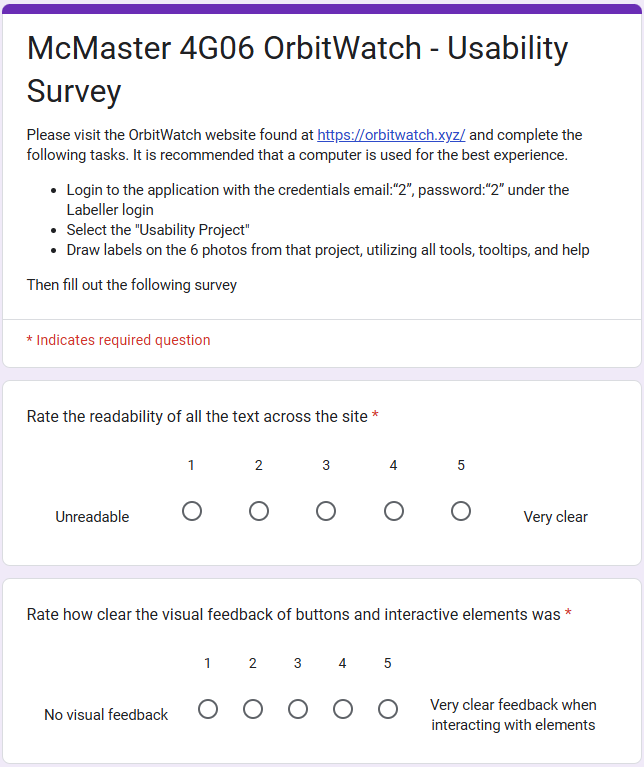
\includegraphics[scale=0.7]{Survey (3).png}\\
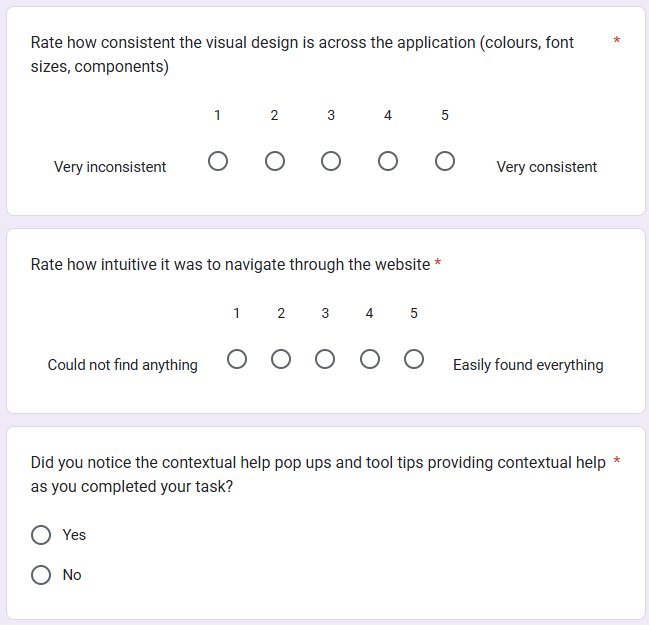
\includegraphics[scale=0.7]{Survey (4).png}\\
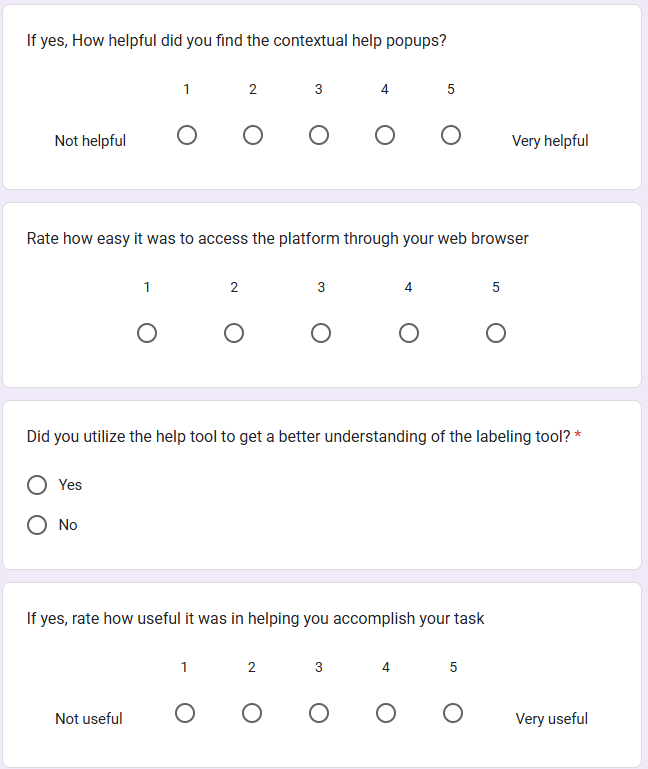
\includegraphics[scale=0.7]{Survey (1).png}\\
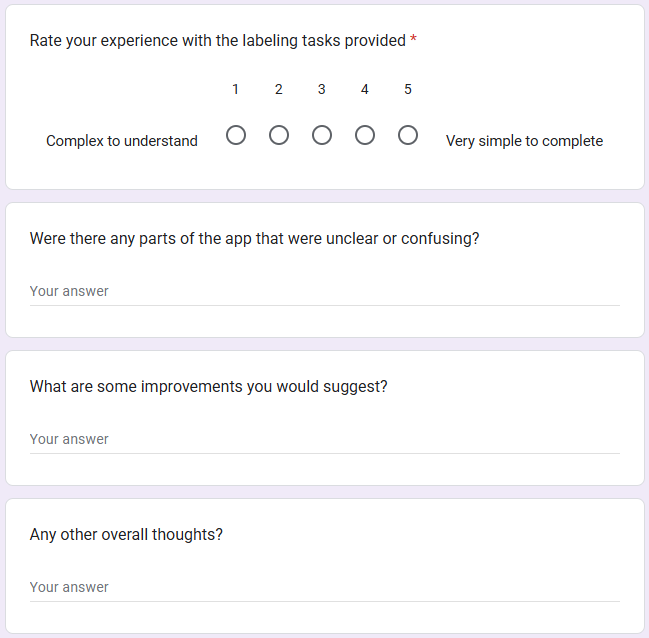
\includegraphics[scale=0.7]{Survey (2).png}\\
\end{centering}
Each of the testers is aged 20-26, university educated, and familiar with technology. We understand this to be a limitation of our experiment, as ideally we would have access to testers from a wider range of ages, backgrounds, and expertise. However, we believe the result from this 
survey remain valuable to identify areas for improvement for our website's usability.
\subsection{Results}
After conducting the survey, we have received the following results.
\begin{centering}
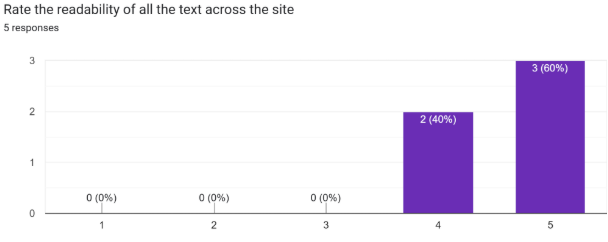
\includegraphics[scale=0.7]{chart (2).png}\\
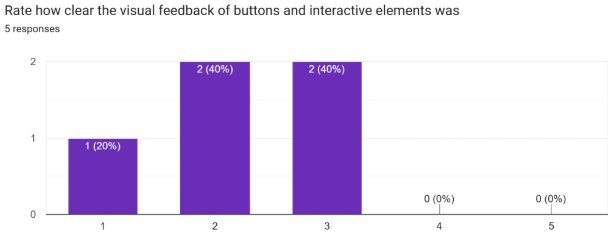
\includegraphics[scale=0.7]{chart (3).png}\\
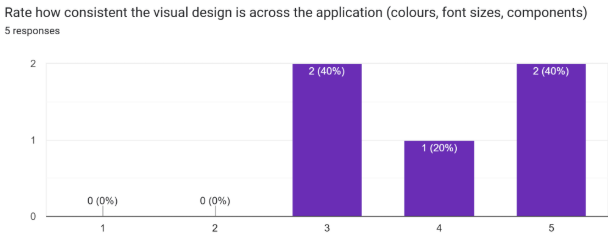
\includegraphics[scale=0.7]{chart (4).png}\\
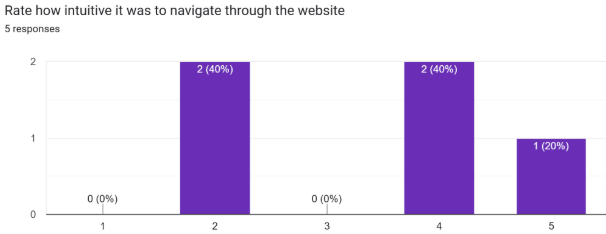
\includegraphics[scale=0.7]{chart (5).png}\\
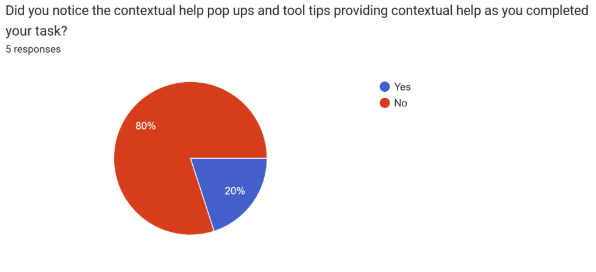
\includegraphics[scale=0.7]{chart (6).png}\\
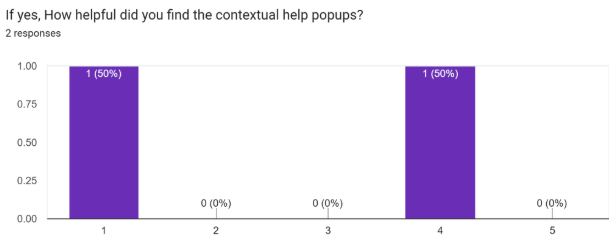
\includegraphics[scale=0.7]{chart (7).png}\\
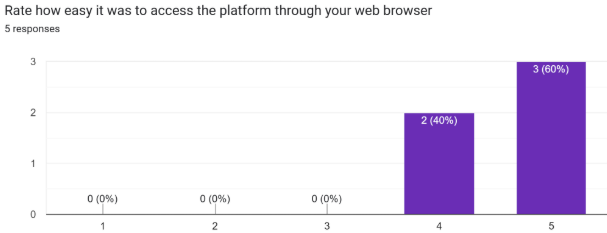
\includegraphics[scale=0.7]{chart (8).png}\\
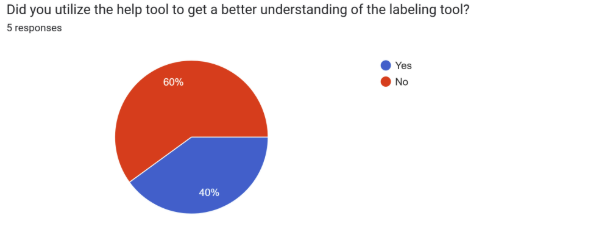
\includegraphics[scale=0.7]{chart (9).png}\\
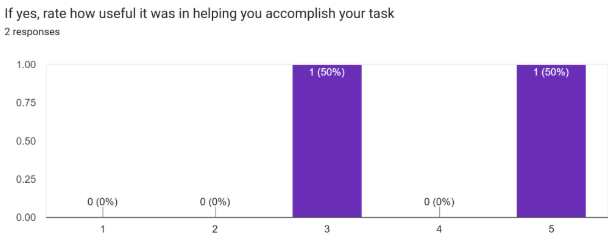
\includegraphics[scale=0.7]{chart (10).png}\\
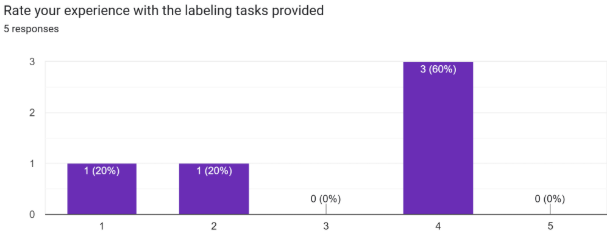
\includegraphics[scale=0.7]{chart (1).png}\\
\end{centering}
We also obtained qualitative feedback, which will be discussed in the analysis section.
\subsection{Analysis}
From these results, some obvious trends emerge. First, readability and design are the current strong points. Most people agree that the text is readable, and the design is consistent. This is critical for improving the discoverability of the site.
Unfortunately, there are quite a few more areas for improvement. Several of the respondents reported that it was challenging to know what to do. They were unaware of the purpose of the website and of the features available to them. One user commented `The overall concept of the application was slightly confusing, the help button did aid in learning what to do. I thought I was only allowed to label once, before realizing I have to select the same label button multiple times.'
It is very important that we ensure new users are able to complete tasks easily. Otherwise, we may lose users to frustration. One user suggested including a `3-second gif' of someone labeling a similar image before a user labels for the first time. This would likely be enough to eliminate a lot of confusion from the users. Another area for improvement is related to feedback when labelling. Several users were unsure when a label was submitted, or what buttons like `skip' or `next' do. 
This will again lead to frustration and confusion, alienating users. 

\subsection{Next Steps}
We will implement the feedback collected in this first survey to improve the site for Rev1. After changes have been implemented, we will redistribute the survey to the same testers. We are hoping to see an improvement in the rating collected between the first and second survey.
 

\section{Additional Survey}

\end{document}
